קיימים שני ייצוגים סטנדרטים של גרפים (מכוונים או לא):
\begin{enumerate}
\item
על ידי מטריצת שכנויות
\item
על ידי רשימת שכנויות
\end{enumerate}
אם לא מצוין אחרת, נניח שהגרף מיוצג על ידי רשימת שכנויות.
\\
למשל את הגרף:
\begin{center}
\begin{tikzpicture}[every node/.style={default node}]
\foreach[count=\i] \x/\y in {
	0/0
	,1/1
	,1/-1
	,2/0
}{
\node(\i) at(\x,\y) {\i};
}
\foreach \u/\v in {%
	1/2%
	,2/4%
	,1/4%
	,3/4%
}{
	\draw[->] (\u) -- (\v)
}
\end{tikzpicture}
\end{center}
ניתן לייצג על ידי המטריצה 
\begin{center}
\begin{bmatrix}
0 & 1 & 0 & 1
\\
0 & 0 & 0 & 1
\\
0 & 0 & 0 & 1
\\
0 & 0 & 0 & 0
\end{bmatrix}
\end{center}
וגם על ידי רשימת שכנויות:
\begin{center}
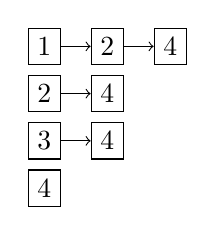
\begin{tikzpicture}[every node/.style={rectangle, draw}, y=6mm, x=8mm]
\foreach[count=\i] \x\y\n in {
	0/0/1
	,0/-1/2
	,0/-2/3
	,0/-3/4	
	%
	,1/0/2
	,2/0/4
	%
	,1/-1/4
	%
	,1/-2/4	
}{
	\node(\i) at(\x,\y){\n};
}
\foreach \u\v in {%
	1/5%
	,5/6%
	,2/7%
	,3/8%
}{
\draw[->] (\u) -- (\v);
}
\end{tikzpicture}
\end{center}




